%%%%%%%%%%%%%%%%%%%%%%%%%%%%%%%%%%%%%%%%%
% Programming/Coding Assignment
% LaTeX Template
%
% This template has been downloaded from:
% http://www.latextemplates.com
%
% Original author:
% Ted Pavlic (http://www.tedpavlic.com)
%
% Note:
% The \lipsum[#] commands throughout this template generate dummy text
% to fill the template out. These commands should all be removed when 
% writing assignment content.
%
% This template uses a Perl script as an example snippet of code, most other
% languages are also usable. Configure them in the "CODE INCLUSION 
% CONFIGURATION" section.
%
%%%%%%%%%%%%%%%%%%%%%%%%%%%%%%%%%%%%%%%%%

%----------------------------------------------------------------------------------------
%	PACKAGES AND OTHER DOCUMENT CONFIGURATIONS
%----------------------------------------------------------------------------------------

\documentclass{article}
\usepackage{fancyhdr} % Required for custom headers
\usepackage{lastpage} % Required to determine the last page for the footer
\usepackage{extramarks} % Required for headers and footers
\usepackage[usenames,dvipsnames]{color} % Required for custom colors
\usepackage{graphicx} % Required to insert images
\usepackage{caption}
\usepackage{listings} % Required for insertion of code
\usepackage{courier} % Required for the courier font
\usepackage{lipsum} % Used for inserting dummy 'Lorem ipsum' text into the template
\usepackage[colorlinks=true,linkcolor=black,anchorcolor=black,citecolor=black,menucolor=black,runcolor=black,urlcolor=black,bookmarks=true]{hyperref}
\usepackage[table,svgnames]{xcolor}
\usepackage{tabularx}
\usepackage{booktabs}
\usepackage{natbib}

% Margins
\topmargin=-0.45in
\evensidemargin=0in
\oddsidemargin=0in
\textwidth=6.5in
\textheight=9.0in
\headsep=0.25in

\linespread{1.1} % Line spacing

% Set up the header and footer
\pagestyle{fancy}
\lhead{\hmwkAuthorName} % Top left header
\chead{\hmwkClass\ (\hmwkClassInstructor\ \hmwkClassTime): \hmwkTitle} % Top center head
\rhead{\firstxmark} % Top right header
\lfoot{\lastxmark} % Bottom left footer
\cfoot{} % Bottom center footer
\rfoot{Page\ \thepage\ of\ \protect\pageref{LastPage}} % Bottom right footer
\renewcommand\headrulewidth{0.4pt} % Size of the header rule
\renewcommand\footrulewidth{0.4pt} % Size of the footer rule

\setlength\parindent{0pt} % Removes all indentation from paragraphs

%----------------------------------------------------------------------------------------
%	CODE INCLUSION CONFIGURATION
%----------------------------------------------------------------------------------------

\definecolor{MyDarkGreen}{rgb}{0.0,0.4,0.0} % This is the color used for comments
\lstloadlanguages{Perl} % Load Perl syntax for listings, for a list of other languages supported see: ftp://ftp.tex.ac.uk/tex-archive/macros/latex/contrib/listings/listings.pdf
\lstset{language=Perl, % Use Perl in this example
        frame=single, % Single frame around code
        basicstyle=\small\ttfamily, % Use small true type font
        keywordstyle=[1]\color{Blue}\bf, % Perl functions bold and blue
        keywordstyle=[2]\color{Purple}, % Perl function arguments purple
        keywordstyle=[3]\color{Blue}\underbar, % Custom functions underlined and blue
        identifierstyle=, % Nothing special about identifiers                                         
        commentstyle=\usefont{T1}{pcr}{m}{sl}\color{MyDarkGreen}\small, % Comments small dark green courier font
        stringstyle=\color{Purple}, % Strings are purple
        showstringspaces=false, % Don't put marks in string spaces
        tabsize=5, % 5 spaces per tab
        %
        % Put standard Perl functions not included in the default language here
        morekeywords={rand},
        %
        % Put Perl function parameters here
        morekeywords=[2]{on, off, interp},
        %
        % Put user defined functions here
        morekeywords=[3]{test},
       	%
        morecomment=[l][\color{Blue}]{...}, % Line continuation (...) like blue comment
        numbers=left, % Line numbers on left
        firstnumber=1, % Line numbers start with line 1
        numberstyle=\tiny\color{Blue}, % Line numbers are blue and small
        stepnumber=5 % Line numbers go in steps of 5
}

% Creates a new command to include a perl script, the first parameter is the filename of the script (without .pl), the second parameter is the caption




%----------------------------------------------------------------------------------------
%	DOCUMENT STRUCTURE COMMANDS
%	Skip this unless you know what you're doing
%----------------------------------------------------------------------------------------

% Header and footer for when a page split occurs within a problem environment
\newcommand{\enterProblemHeader}[1]{
\nobreak\extramarks{#1}{#1 continued on next page\ldots}\nobreak
\nobreak\extramarks{#1 (continued)}{#1 continued on next page\ldots}\nobreak
}

% Header and footer for when a page split occurs between problem environments
\newcommand{\exitProblemHeader}[1]{
\nobreak\extramarks{#1 (continued)}{#1 continued on next page\ldots}\nobreak
\nobreak\extramarks{#1}{}\nobreak
}

\setcounter{secnumdepth}{0} % Removes default section numbers
\newcounter{homeworkProblemCounter} % Creates a counter to keep track of the number of problems

\newcommand{\homeworkProblemName}{}
\newenvironment{homeworkProblem}[1][Problem \arabic{homeworkProblemCounter}]{ % Makes a new environment called homeworkProblem which takes 1 argument (custom name) but the default is "Problem #"
\stepcounter{homeworkProblemCounter} % Increase counter for number of problems
\renewcommand{\homeworkProblemName}{#1} % Assign \homeworkProblemName the name of the problem
\section{\homeworkProblemName} % Make a section in the document with the custom problem count
\enterProblemHeader{\homeworkProblemName} % Header and footer within the environment
}{
\exitProblemHeader{\homeworkProblemName} % Header and footer after the environment
}

\newcommand{\problemAnswer}[1]{ % Defines the problem answer command with the content as the only argument
\noindent\framebox[\columnwidth][c]{\begin{minipage}{0.98\columnwidth}#1\end{minipage}} % Makes the box around the problem answer and puts the content inside
}

\newcommand{\homeworkSectionName}{}
\newenvironment{homeworkSection}[1]{ % New environment for sections within homework problems, takes 1 argument - the name of the section
\renewcommand{\homeworkSectionName}{#1} % Assign \homeworkSectionName to the name of the section from the environment argument
\subsection{\homeworkSectionName} % Make a subsection with the custom name of the subsection
\enterProblemHeader{\homeworkProblemName\ [\homeworkSectionName]} % Header and footer within the environment
}{
\enterProblemHeader{\homeworkProblemName} % Header and footer after the environment
}

%----------------------------------------------------------------------------------------
%	NAME AND CLASS SECTION
%----------------------------------------------------------------------------------------

\newcommand{\hmwkTitle}{A3} % Assignment title
\newcommand{\hmwkDueDate}{Thursday,\ February\ 23,\ 2017} % Due date
\newcommand{\hmwkClass}{\ INTRO. TO WEB SCIENCE:\ CS 532} % Course/class
\newcommand{\hmwkClassTime}{} % Class/lecture time
\newcommand{\hmwkClassInstructor}{Dr. Nelson} % Teacher/lecturer
\newcommand{\hmwkAuthorName}{Udochukwu Nweke} % Your name

%----------------------------------------------------------------------------------------
%	TITLE PAGE
%----------------------------------------------------------------------------------------

\title{
\vspace{2in}
\textmd{\textbf{\hmwkClass:\ \hmwkTitle}}\\
\normalsize\vspace{0.1in}\small{Due\ on\ \hmwkDueDate}\\
\vspace{0.1in}\large{\textit{\hmwkClassInstructor\ \hmwkClassTime}}
\vspace{3in}
}

\author{\textbf{\hmwkAuthorName}}
\date{} % Insert date here if you want it to appear below your name

%----------------------------------------------------------------------------------------

\begin{document}

\maketitle

%----------------------------------------------------------------------------------------
%	TABLE OF CONTENTS
%----------------------------------------------------------------------------------------

%\setcounter{tocdepth}{1} % Uncomment this line if you don't want subsections listed in the ToC

\newpage
\tableofcontents
\newpage

%----------------------------------------------------------------------------------------
%	PROBLEM 1
%----------------------------------------------------------------------------------------

% To have just one problem per page, simply put a \clearpage after each problem

\begin{homeworkProblem}

1. Download the 1000 URIs from assignment \# 2. ``curl'', ``wget'', or ``lynx'' are all good candidate programs to use. We want just the raw raw HTML, not images, stylesheets, etc.
Listing shows a Perl script.

\lstinputlisting[caption=Extract HTML, language=python]{P1.py}
\textbf{Solution 1:}\\
 1.   In order to get the raw HTML files for the 1000 files I downloaded from Assignment \#2,I used a function called  \textit{derefURL()} to extract the HTML contents using curl -L option to follow redirects. The raw HTML for the 1000 URIs is saved in RawHTML folder. This can be seen in listing 1 line 39 


2. After downloading the HTML files, I used NLTK clean HTML function \textit{(clean-html())} remove the HTML markup.
  This is seen in Listing 1, line 12.

 \begin{table}[h!]
  \centering
  \caption{10 Hits for the term ``Russia'', ranked by TFIDF. Complete URL list in file``10URLsWithRussia.txt''}
  \label{tab:idf}
  \begin{tabular}{cccl}
    \toprule
      TFIDF   & TF   & IDF  &URI \\
    \midrule
    0.0151 & 0.0044  & 3.4226  &\url{http://insider.foxnews.com/...}\\
    0.0041 & 0.0012  & 3.4226  &\url{http://variety.com/...}\\
    0.0038& 0.0011   & 3.4266  & \url{http://www.express.co.uk/...}\\
    0.0034& 0.0001   & 3.4266  & \url{http://100percentfedup.com/...}\\
    0.0027& 0.0008   & 3.4266  & \url{http://www.latimes.com/...}\\
    0.0027& 0.0008   & 3.4266  & \url{http://www.politico.com/...}\\
    0.0024& 0.0007   & 3.4266  & \url{https://www.buzzfeed.com/...}\\
    0.0017& 0.0005   & 3.4266  & \url{https://www.washingtonpost.com/...}\\
    0.0017& 0.0005   & 3.4266  & \url{https://www.theatlantic.com/...}\\
    0.0014& 0.0004   & 3.4266  & \url{http://www.ocregister.com/...}\\


    \bottomrule
  \end{tabular}
\end{table}

\end{homeworkProblem}

%----------------------------------------------------------------------------------------
%	PROBLEM 2
%----------------------------------------------------------------------------------------



\begin{homeworkProblem}

Choose a query term (e.g., ``Shadow'') that is not a stop word (see week 5 slides) and not the HTML markup from step 1 (e.g. ``http'') that matches at least 10 documents (hint: use ``grep'' on the processed files). If the term is present in more than 10 documents, choose any 10 from your list. (If you do not end up with 10 documents, you've done something wrong).\\

As per the example in the week 5 slides, compute TFIDf values for the term in each of the 10 documents and create a table with the TF, IDF, and TFIDF values, as well as the corressponding URIs. The URIs will be ranked in decreasing order by TFIDF values. 
\lstinputlisting[caption= TFIDF Code Snippet,language=python]{P2.py}

\textbf{Solution 2:}\\
1. I chose a query term ``Russia'' and used grep command to search the number of times term ``Russia'' appeared in 10 different documents. 
grep-i gave me the flexibility of searching for both upper and lower case terms. grep -w is to match the whole word so as not to match sub strings. For example, don't match ``Russian'', but match ``Russia''. The function \textit{searchForTermInFiles()} in line 7 of listing 2. is used to search for  term``Russia'' in the files.\\


2. After searching for term ``Russia'' and calculating the number of times it appeared in the document, I created a function to calculate the TFIDF. The function \textit{calculateTFIDFForIndex()} is the fuction that calculates the TFIDF for all 10 documents with term ``Russia''.\\

TFIDF is the product of TF and IDF

TF is the Term Frequency and it counts the number of times term ``Russia'' occurs in the document. I got 93 documents with  term ``Russia'' out of 1000 documents.
IDF is the inverse Document Frequency and is calculated as follows:\\
             
             $IDF = \frac{Number of documents}{Number of documents with term Russia} = \frac{1000}{93} = 3.4266$

Table \ref{tab:idf} includes the TFIDF values for all 10 links.
\end{homeworkProblem}



%----------------------------------------------------------------------------------------
%PROBLEM 3
%----------------------------------------------------------------------------------------
\begin{homeworkProblem}
Now rank the same 10 URIs from question \#2, but this time 
by their PageRank.  Use any of the free PR estimaters on the web,
such as:

\url{http://pr.eyedomain.com/}\

\url{http://www.prchecker.info/check_page_rank.php}\

\url{http://www.seocentro.com/tools/search-engines/pagerank.html}\

\url{http://www.checkpagerank.net/}\\

If you use these tools, you'll have to do so by hand (they have
anti-bot captchas), but there are only 10 to do.  Normalize the
values they give you to be from 0 to 1.0.  Use the same tool on all
10 (again, consistency is more important than accuracy).  Also
note that these tools typically report on the domain rather than
the page, so it's not entirely accurate.\\




\begin{table}[h!]
  \centering
  \caption{10 Hits for the term ``Russia'', ranked by PageRank}
  \label{tab:pr}
  \begin{tabular}{ccl}
    \toprule
   PageRank Normalised       & PageRank              &URI \\
    \midrule
      1.0                    & 8              &\url{http://insider.foxnews.com/...}\\
      1.0                    & 8              & \url{http://www.latimes.com/...}\\
      1.0                    & 8              & \url{https://www.buzzfeed.com/...}\\
      1.0                    & 8              & \url{https://www.washingtonpost.com/...}\\
      1.0                    & 8              & \url{https://www.theatlantic.com/...}\\
      0.9                    & 7              &\url{http://variety.com/...}\\
      0.9                    & 7              & \url{http://www.express.co.uk/...}\\
      0.9                    & 7              & \url{http://www.politico.com/...}\\
      0.9                    & 6              & \url{http://www.ocregister.com/...}\\
      0.0                    & 0              & \url{http://100percentfedup.com/...}\\

    \bottomrule
  \end{tabular}
\end{table}

\begin{table}[h!]
  \centering
  \caption{10 Hits for the term ``Russia'', ranked by AlexaRank}
  \label{tab:pr}
  \begin{tabular}{cl}
    \toprule
   AlexaRank               &URI \\
    \midrule
      135                  &\url{https://www.washingtonpost.com/}\\
      202                 & \url{https://www.buzzfeed.com/}\\
      261                 & \url{http://insider.foxnews.com/}\\
      845                 & \url{http://www.latimes.com/}\\
      901                 & \url{http://www.politico.com/}\\
      1156                &\url{https://www.theatlantic.com/}\\
      1191                & \url{http://www.express.co.uk/}\\
      2462                & \url{http://variety.com/}\\
      15728               & \url{http://www.ocregister.com/}\\
      30729               & \url{http://100percentfedup.com/}\\

    \bottomrule
  \end{tabular}
\end{table}

\textbf{Solution 3:}\\
1. Table 2 shows the Page Rank and normalized page rank for the 10 urls.\\

2. I used the \url{http://pr.eyedomain.com/}\\ to get the page ranking for the 10 urls.\\ 

3. Comparing the rankings produced in Table \ref{tab:idf} and \ref{tab:pr} shows that not all urls with high TFIDF have high page ranking.\\

The complete url for Table 1 in in 10CompleteUrl.txt file.
\end{homeworkProblem}

%----------------------------------------------------------------------------------------
%PROBLEM 4
%----------------------------------------------------------------------------------------
\begin{homeworkProblem}

4.  Compute the Kendall Tau\_b score for both lists (use ``b'' because
there will likely be tie values in the rankings).  Report both the
Tau value and the ``p'' value.

\textbf{Solution 4:}\\
1. Table  \ref{tab:ranks} includes the ranks from TFIDF and Page Rank for the list of 10 URLs.\\

2. I computed the Kendall Tau\_b and Pearson correlation coefficient through an R script (Listing 3).\\
 The Kendell Tau\_b value for TFIDF and Page Rank listings is $-0.0809$, and the Pearson Value is $-0.03808$, showing no significant correlations.
 \lstinputlisting[caption= R Code Snippet For Kendell Tau\_b and P values,language=python]{P4.r}

 \begin{table}[h!]
 \centering
 \caption{10 Hits for the term ``Russia'', ranked by PageRank}
  \label{tab:ranks}
  \begin{tabular}{ | l | l | }
  \hline
 TFIDF\_Rank & Page\_Rank \\
 \hline
 1 & 1 \\
 \hline
 2 & 6 \\
 \hline
 3 & 6 \\
 \hline
 4 & 10 \\
 \hline
 5 & 1 \\
 \hline
 5 & 6 \\
 \hline
 7 & 1 \\
 \hline
 8 & 1  \\
 \hline
 8 & 1 \\
 \hline
 10 & 9 \\
 \hline

  \end{tabular}
  \end{table}
\end{homeworkProblem}

%----------------------------------------------------------------------------------------
%PROBLEM 4
%----------------------------------------------------------------------------------------
\begin{homeworkProblem}
Compute a ranking for the 10 URIs from Q2 using Alexa information
(see week 4 slides).  Compute the correlation (as per Q4) for all
pairs of combinations for TFIDF, PR, and Alexa.

\textbf{Solution 5:}\\
1. In order to get the Alexa\_Ranking (Table \ref{tab:alexa}) for the 10 URLs I used Alexa's XML API \url{http://data.alexa.com/data?cli=10&url=}\ to manually get the Alexa\_Rank for the 10 urls (Table \ref{tab:rawalexaRanks}).\\

2. After getting Alexa ranks for the 10 URLs, I used the the values of TFIDF\_Rank, Page\_Rank and Alexa\_Rank to compute the correlation and Kendell Tau\_b values for all combinations through and R script (Listing 3.). Table \ref{tab:correlRanks} displays the Kendall's Tau\_b and P values for all combinations of rankings.

  \begin{table}[h!]
 \centering
 \caption{Alexa\_Rank}
  \label{tab:alexa}
  \begin{tabular}{ | l | l | l|}
  \hline
 TFIDF\_Rank & Page\_Rank  & Alexa\_Rank\\
 \hline
 1 & 1 & s \\
 \hline
 2 & 6 & 8\\
 \hline
 3 & 6 & 7 \\
 \hline
 4 & 10 & 10 \\
 \hline
 5 & 1 & 4 \\
 \hline
 5 & 6 & 5 \\
 \hline
 7 & 1 & 2\\
 \hline
 8 & 1  & 1 \\
 \hline
 8 & 1 & 6 \\
 \hline
 10 & 9 & 9 \\
 \hline

  \end{tabular}
  \end{table}
 \begin{table}[h!]
 \centering
 \caption{Correlation for all pairs of ranks}
  \label{tab:correlRanks}
  \begin{tabular}{ | l | l | l|}
  \hline
 Combination & P-value & Kendall's Tau\_b\\
 \hline
 TFIDF, PR & -0.03805454 & -0.08087458 \\
 \hline
 TFIDF, Alexa& -0.08203403& -0.1136657 \\
 \hline
 PR, Alexa & 0.8731077 & 0.7905694 \\
 \hline
 

  \end{tabular}
  \end{table}

\end{homeworkProblem}
%----------------------------------------------------------------------------------------
%PROBLEM 4
%----------------------------------------------------------------------------------------
\begin{homeworkProblem}
6.  Give an in-depth analysis, complete with examples, 
graphs, and all other pertinent argumentation for 
Kristen Stewart's (of ``Twilight'' fame) Erdos\-Bacon number.\\

\textbf{Solution 6:}\\
``Six Degrees of Separation'' is the name of an academic play by John Guarre. This concept creates a place that would connect millions of people around the world. This concept explains how anyone in the planet can be connected to another person with an average of six jumps. Hence, the society we live in is a small\-world type of network characterised by short path lengths.\\

``Six degrees of Kavin Bacon'' is a palour game for movie lovers. The Bacon number of a movie actor tries to connect a particular actor to Kavin Bacon. The number of jumps it takes to link a particular actor to a movie with Kavin Bacon directly or indirectly will give the actor's Bacon number. Directly means that the actor has appeared in the same movie with Kavin Bacon, while indirectly means the actor has appeared in a movie with some actor that has appeared in a movie with Kavin Bacon.\\

Just as ``Six degrees of Kavin Bacon'' is used to get an actor’s Bacon number, the Erdos number also gives the collaborative distance between mathematician Paul Erdos and some other person. The Erdos number can be measured by authorship of mathematical papers. Hence, Erdos number is the jumps it takes to link an author who co-authored with Paul Erdos directly or indirectly. \\

Erdos-Bacon number is simply the sum of Bacon number and Erdos number.\\

Kristen Stewarts Erdos-Bacon number will be the sum of the jumps it takes to link her to to a movie with Kevin Bacon directly or indirectly (Bacon number) and the jumps it takes to link her with a publication co-authored with Paul Erdon directly or indirectly (Erdos number). I used 
\url{https://oracleofbacon.org/} to calculate how Kristen Stewart is linked to kavin Bacon via movie appearances (Figure 1.) She has a Bacon number of 2.

In order to calculate Kristen Stewart's erdos number, I looked for a co-author that connected her to Paul Erdos indirectly.  She published a paper on ``Bringing Imression to Life with Neural Style Transfer in Come Swim'' with Bautik J Josheni and David Shapiro. I searched for Bhautik's publications and found out that Bhautik co-authored most of his publications with Sebastein Ourselin and Sebastin Ourselin has an erdos number of 4 as shown in figure 2. This gives Kristen Stewart an Erdos number of 6.\\

The graph in figure 3 shows one of several links from Kristen Stewart to Paul Erdos based on paper publication.

However, there could be possible shorter links from Kristen Stewart, but this will require an exhaustive exploration of authorship graph.  Figure 4 shows an imaginary graph with possible shorter links to Erdos.

Kristen Stewart's Erdos-Bacon number is 2+6 = 8.

\begin{center}
  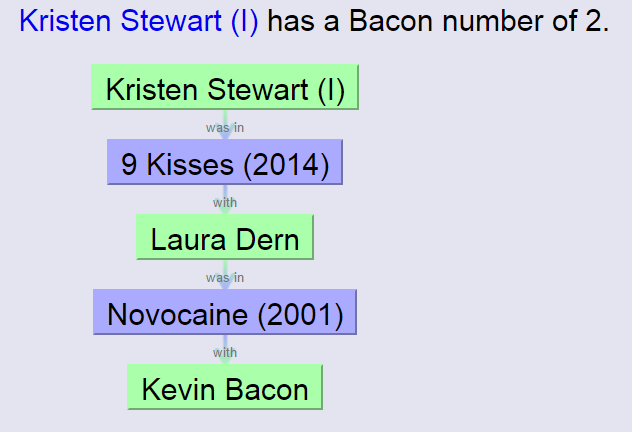
\includegraphics{baconnumber.png}
  \captionof{figure} {Bacon Number Result }
\end{center}


\begin{center}
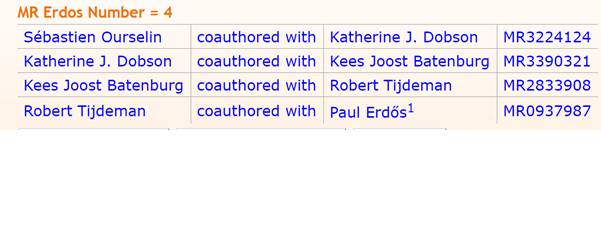
\includegraphics{erdosnumber.png}
\captionof{figure} {Erdos Number Result}
\end{center}


\begin{center}
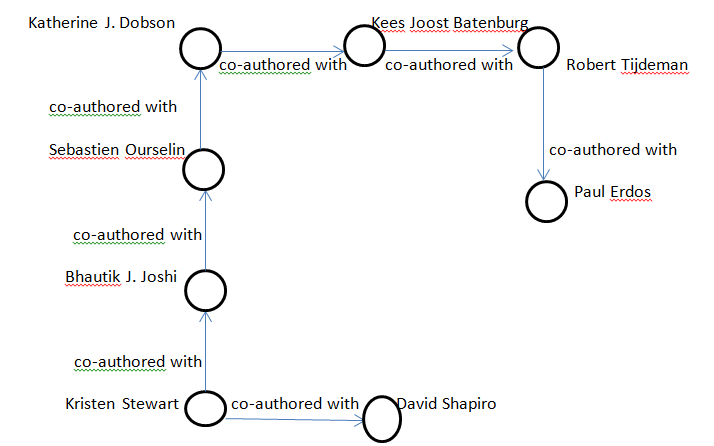
\includegraphics{Erdos_Grapg.png}
\captionof{figure} {Kristen Stewart's Erdos Graph }
\end{center}


\begin{center}
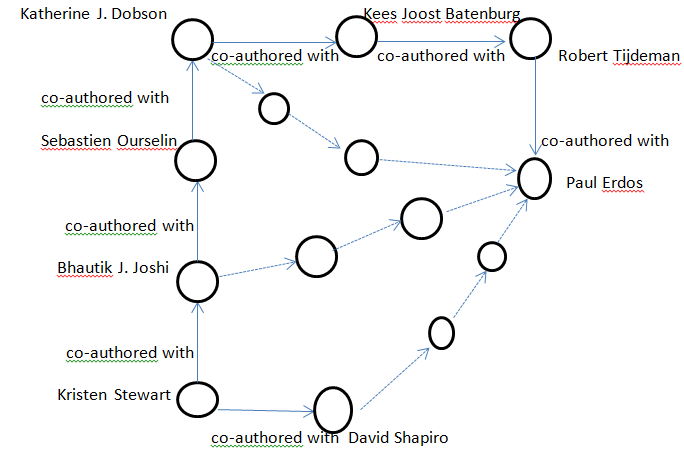
\includegraphics{ErdosImaginary_Graph2.png}
\captionof{figure} {Kristen Stewart's Erdos Imaginary Graph }
\end{center}

\end{homeworkProblem}

%----------------------------------------------------------------------------------------
%PROBLEM 7
%----------------------------------------------------------------------------------------
\begin{homeworkProblem}
Build a simple (i.e., no positional information) inverted file
(in ASCII) for all the words from your 1000 URIs.  Upload the entire
file to github and discuss an interesting portion of the file in
your report. 

\textbf{Solution 7:}\\
\lstinputlisting[caption= Inverted File Code,language=python]{P7_optimized.py}

In order to generate an inverted file, I created a giant dictionary which consists of all terms in all the documents and I tokenised by space. I checked how many documents had each term in the vocabulary and wrote this statistic for each term.
The inverted file text is in InvetedFile\_good text folder
The ``stop words'' have the highest nuber of appearance in the document.
\end{homeworkProblem}

\nocite{*}
\bibliographystyle{plain}
\bibliography{A3Ref}

\end{document}